
\section{Erweiterte \stmt{WENN} Funktionen}

\subsection{\stmt{SUMMEWENN} Funktion}

Mit dieser Funktion kann man in Zellbereichen numerische Werte addieren, die bestimmten Bedingungen in gleichen oder anderen Zellbereichen unterworfen sind.%
$$ \text{\stmt{WENN(\syntax{Bereich}; \syntax{Suchkriterien}; \syntax{SUMME\_BEREICH})}}$$%
%
Das folgende Beispiel zeigt die Umsätze in Abhängigkeit der Kategorie%
	\begin{figure}[H]
		\centering
%			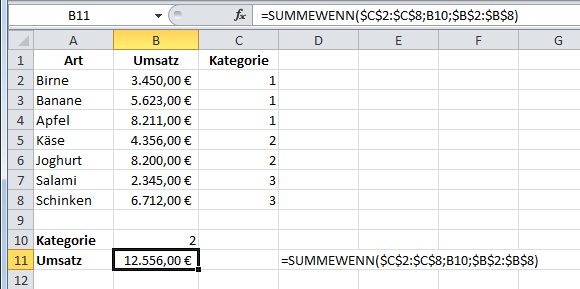
\includegraphics[width=10cm]{images/summewenn}
			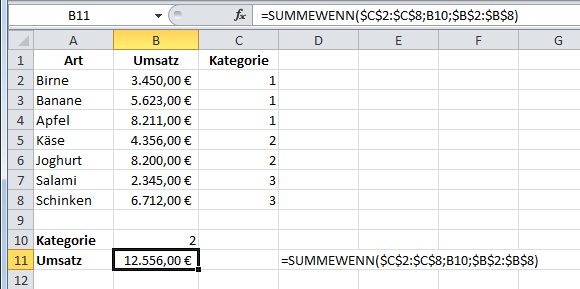
\includegraphics[scale=0.7]{images/summewenn}
		\caption{\stmt{SUMMEWENN} Funktion}
		\label{fig:summewenn}
	\end{figure}

\subsection{\stmt{SUMMEWENNS} Funktion}

Bei dieser Funktion kann man Werte addieren, welche anhand von bis zu 127 Kriterien gefilter wurden

$$ \text{\stmt{WENN(\syntax{Summe\_Bereich}; \syntax{Kriterien\_Bereich1}; \syntax{Kriterien1}; \ldots)}}$$%
%
\begin{description}[labelindent=0cm, leftmargin=4cm, font=\mdseries, labelwidth=3cm,style=nextline]
\smallitemize
\item[\syntax{Summe\_Bereich}] Jener Zellbereich, der summiert werden soll.
\item[\syntax{Kriterien\_Bereich1}] Jener Zellbereich, auf den das Kriterium $(n)$ angewendet werden soll.
\item[\syntax{Kriterien1}] Jene Suchbedingung, die auf den Kriterien Bereich $(n)$ angewendet werden soll.
\end{description}

\figref{fig:summewenns} zeigt die Umsätze in Abhängigkeit der Kategorie und eines Zeitraumes%
	\begin{figure}[H]
		\centering
%			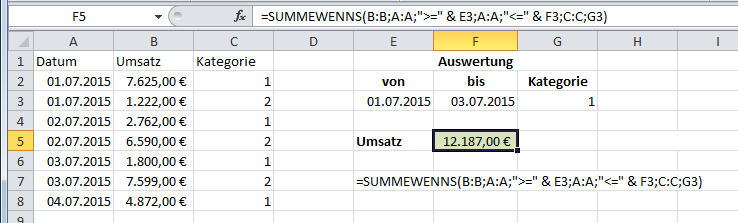
\includegraphics[width=14cm]{images/summewenns}
			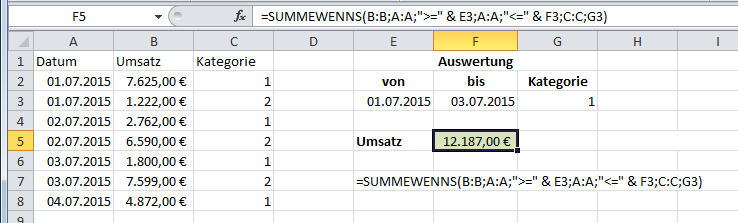
\includegraphics[scale=0.7]{images/summewenns}
		\caption{\stmt{SUMMEWENNS} Funktion}
		\label{fig:summewenns}
	\end{figure}



\subsection{\stmt{ZÄHLENWENN} Funktion}

Mit dieser Funktion kann man die Anzahl der zutreffenden Zellen zählen, die bestimmten Bedingungen entsprechen.%
$$ \text{\stmt{WENN(\syntax{Bereich}; \syntax{Suchkriterien}; \syntax{SUMME\_BEREICH})}}$$%
%
Das folgende Beispiel zeigt die Umsätze in Abhängigkeit der Kategorie%
	\begin{figure}[H]
		\centering
%			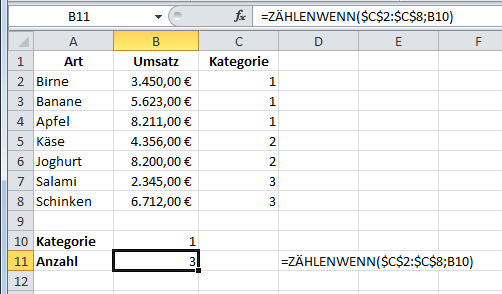
\includegraphics[width=10cm]{images/zaehlenwenn}
			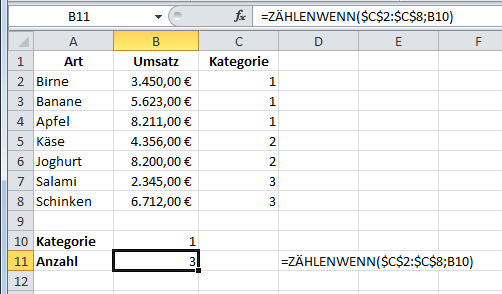
\includegraphics[scale=0.7]{images/zaehlenwenn}
		\caption{\stmt{ZÄHLENWENN} Funktion}
		\label{fig:zaehlenwenn}
	\end{figure}

\subsection{\stmt{ZÄHLENWENNS} Funktion}

Bei dieser Funktion kann man Werte zählen, welche anhand von bis zu 127 Kriterien gefiltert wurden

$$ \text{\stmt{WENN(\syntax{Summe\_Bereich}; \syntax{Kriterien\_Bereich1}; \syntax{Kriterien1}; \ldots)}}$$%
%
\begin{description}[labelindent=0cm, leftmargin=4cm, font=\mdseries, labelwidth=3cm,style=nextline]
\smallitemize
\item[\syntax{Summe\_Bereich}] Jener Zellbereich, der summiert werden soll.
\item[\syntax{Kriterien\_Bereich1}] Jener Zellbereich, auf den das Kriterium $(n)$ angewendet werden soll.
\item[\syntax{Kriterien1}] Jene Suchbedingung, die auf den Kriterien Bereich $(n)$ angewendet werden soll.
\end{description}
\pagebreak
\figref{fig:zaehlenwenns} zeigt die Anzahl von Personen, welche in einem bestimmter Altersbereich sind, Raucher sind und Übergewicht haben%
	\begin{figure}[H]
		\centering
%			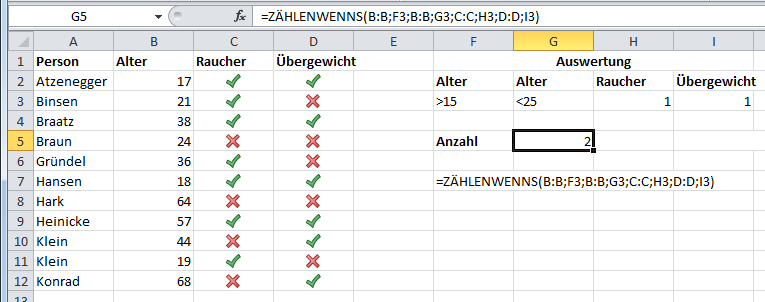
\includegraphics[width=14cm]{images/zaehlenwenns}
			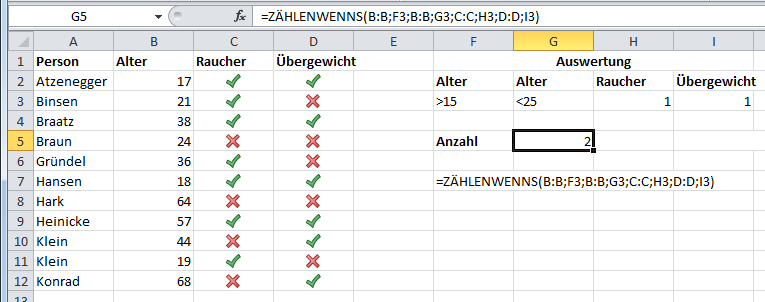
\includegraphics[scale=0.7]{images/zaehlenwenns}
		\caption{\stmt{ZAEHLENWENNS} Funktion}
		\label{fig:zaehlenwenns}
	\end{figure}


